\documentclass[a4paper,12pt,twoside]{report}
\usepackage[left=2cm,right=2cm,top=2cm,bottom=3cm]{geometry}
\usepackage[greek,english]{babel}
\usepackage{amsmath}
\usepackage{graphicx}
\usepackage{float}
\usepackage{listings}
\usepackage{hyperref}
\hypersetup{
    colorlinks=true,
    linkcolor=blue,
    filecolor=blue,
    urlcolor=blue,
}

\setcounter{tocdepth}{3}  
\setcounter{secnumdepth}{3} 

\newcommand{\submitdate}{\gr{Σεπτέμβριος 2024}}

\newcommand{\gr}{\selectlanguage{greek}}
\newcommand{\en}{\selectlanguage{english}}

\renewcommand{\thesection}{\arabic{section}}

\begin{document}

\begin{titlepage}
    \centering
    \includegraphics[width=0.5\textwidth]{images/ionio.png} 
    \vspace{1cm}
    
    {\huge\bfseries \gr{Αναφορά Εργασίας στην Τεχνολογία Λογισμικού}\par} 
    \vspace{2cm}
    
    {\Large \gr{Όνομα: Κωνσταντίνος Καφτεράνης}\par} 
    \vspace{0.5cm}
    
    {\Large \gr{ΑΜ: \en{inf2021090}}\par} 
    \vfill
    
    {\large \submitdate\par} 
\end{titlepage}

\renewcommand{\contentsname}{\gr{Περιεχόμενα}} 
\tableofcontents

\section{\gr{Εισαγωγή}}

\gr{Για την εργασία του μαθήματος Τεχνολογία Λογισμικού, δημιουργήθηκε μια διαδικτυακή εφαρμογή μηχανικής μάθησης για την ανάλυση δεδομένων. Η υλοποίηση πραγματοποιήθηκε με τη γλώσσα προγραμματισμού} \en{Python} \gr{χρησιμοποιώντας τη βιβλιοθήκη} \en{Streamlit} \gr{καθώς και άλλες βιβλιοθήκες μηχανικής μάθησης όπως} \en{Scikit-learn, Pandas} \gr{και} \en{Matplotlib}. \gr{Η εφαρμογή ενσωματώνει διάφορους αλγορίθμους μηχανικής μάθησης για κατηγοριοποίηση και ομαδοποίηση, ενώ προσφέρει δυνατότητες οπτικοποίησης των δεδομένων μέσω γραφημάτων και διαγραμμάτων. Η εφαρμογή παρέχει μια φιλική προς τον χρήστη διεπαφή για τη φόρτωση δεδομένων, την επεξεργασία τους και την εξαγωγή πολύτιμων πληροφοριών μέσω στατιστικής ανάλυσης και οπτικοποίησης.}

\section{\gr{Μεθοδολογία Υλοποίησης - ΚλυκλοςΖωής Λογισμικού}} 

\subsection{\gr{Μοντέλο Επαναληπτικής Ανάπτυξης} \en{(Iterative Model)}}
\gr{Το Μοντέλο Επαναληπτικής Ανάπτυξης είναι μια ευέλικτη προσέγγιση ανάπτυξης λογισμικού που βασίζεται στη συνεχή βελτίωση του λογισμικού μέσα από επαναλαμβανόμενες φάσεις ανάπτυξης.}
\begin{itemize}
    \item \gr{Ξεκινάει με τη συλλογή των απαιτήσεων και την ανάλυση των αναγκών του έργου.}
    \item \gr{Ο κώδικας γράφεται σε μικρές, διαχειρίσιμες μονάδες, με κάθε μονάδα να δοκιμάζεται ξεχωριστά, δίνοντας έμφαση στη διόρθωση λαθών πριν προχωρήσουμε στην επόμενη ενότητα.}
    \item \gr{Η ανάπτυξη γίνεται τμηματικά, με την ολοκλήρωση κάθε μονάδας να συμβάλλει στη συνολική ανάπτυξη του συστήματος.}
    \item \gr{Οι τελικές διορθώσεις και βελτιώσεις γίνονται μόνο όταν το κύριο σύστημα είναι σταθερό και λειτουργικό.}
\end{itemize}
\gr{Αυτή η προσέγγιση επιτρέπει την γρήγορη διόρθωση λαθών και την καλύτερη διαχείριση των απαιτήσεων που μπορεί να αλλάζουν κατά την ανάπτυξη της εφαρμογής.}

\section{\gr{Δομή Εφαρμογής}} 

\begin{figure}[H]
    \centering
    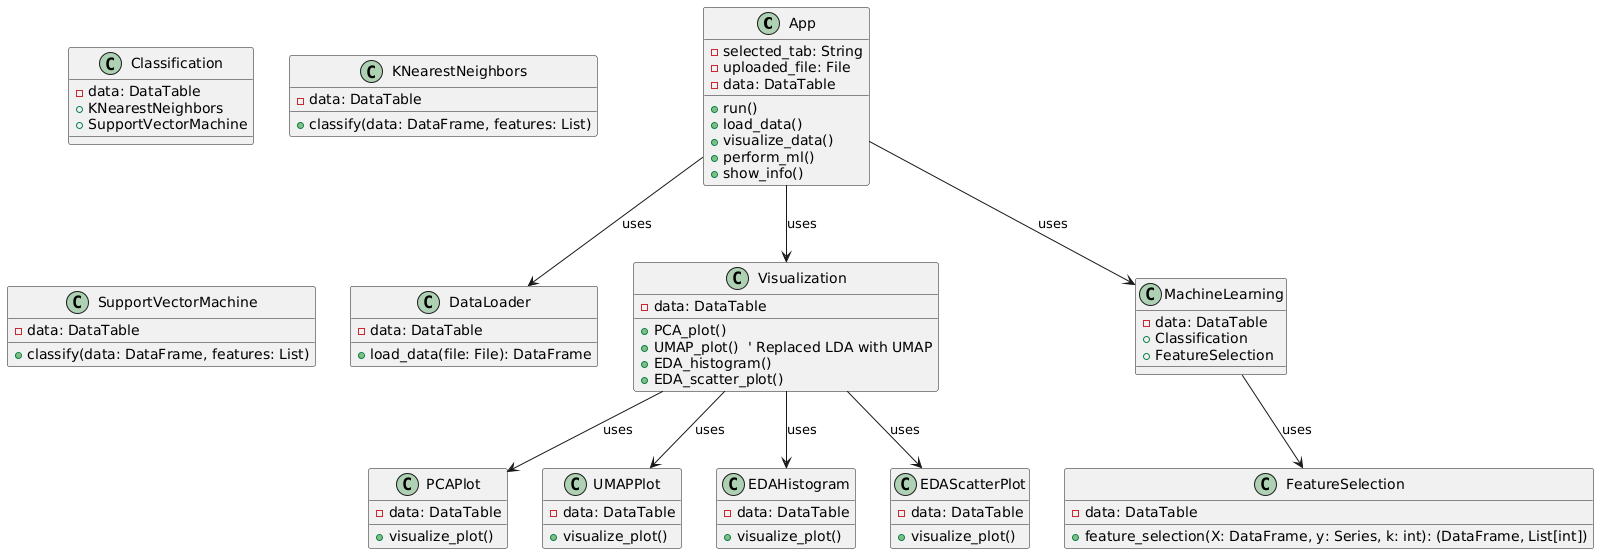
\includegraphics[width=1.25\textwidth]{images/diagra.png} 
    \caption{\gr{Το} \en{UML} \gr{διάγραμμα.}}
%    \label{fig:my_figure} % Optional: 
\end{figure}

\subsection{\en{App}}

\subsubsection{\en{display\_data}}
\begin{itemize}
    \item \gr{Η συνάρτηση} \en{display\_data} \gr{εμφανίζει τον πίνακα δεδομένων στην εφαρμογή.}
    \item \gr{Συγκεκριμένα, χρησιμοποιεί την} \en{st.write} \gr{για να προβάλλει τα δεδομένα στην πλευρική γραμμή της εφαρμογής.}
\end{itemize}

\subsubsection{\en{split\_data}}
\begin{itemize}
    \item \gr{Η συνάρτηση} \en{split\_data} \gr{διαχωρίζει τα δεδομένα σε χαρακτηριστικά (} \en{X} \gr{) και στόχο (} \en{y} \gr{).}
    \item \gr{Τα χαρακτηριστικά περιλαμβάνουν όλες τις στήλες εκτός από την τελευταία, ενώ η τελευταία στήλη θεωρείται η μεταβλητή στόχος.}
    \item \gr{Εμφανίζει τα χαρακτηριστικά και τη μεταβλητή στόχο στην εφαρμογή χρησιμοποιώντας την} \en{st.write} \gr{και επιστρέφει τα} \en{X} \gr{και} \en{y}.
\end{itemize}

\subsubsection{\en{main}}
\begin{itemize}
    \item \gr{Η συνάρτηση} \en{main} \gr{είναι η κύρια συνάρτηση της εφαρμογής και διαχειρίζεται την κύρια ροή της εφαρμογής.}
    \item \gr{Διαχειρίζεται την πλοήγηση μέσω της} \en{sidebar} \gr{της εφαρμογής και καλεί άλλες συναρτήσεις ανάλογα με την επιλεγμένη ενότητα.}
    \item \gr{Η ενότητα} \en{Upload Data} \gr{φορτώνει και εμφανίζει δεδομένα από αρχεία \en{CSV} \gr{ή} \en{Excel.}}
    \item \gr{Η ενότητα} \en{Data Visualization} \gr{επιτρέπει την απεικόνιση των δεδομένων με διάφορους τύπους γραφημάτων, όπως} \en{PCA} \gr{και} \en{UMAP}.
    \item \gr{Η ενότητα} \en{Machine Learning} \gr{εκτελεί αλγορίθμους μηχανικής μάθησης, όπως} \en{KNN} \gr{και} \en{SVM} \gr{για ταξινόμηση} 
    \item \gr{ Η ενώτητα} \en{Feature Selection} \en{επιτρέπει τον χρήστη να επιλέξει ένα αριθμό απο χαρακτηριστικά του σετ για να εφαρμοστούν οι αλγόριθμοι}
    \item \gr{Η ενότητα} \en{Information} \gr{καλεί τη συνάρτηση} \en{display\_info} \gr{για να εμφανίσει πληροφορίες σχετικά με την εφαρμογή.}
\end{itemize}

\subsection{\en{ML}}
\subsubsection{\en{Classification}}
\gr{Η κατηγοριοποίηση είναι η διαδικασία της ανάθεσης μιας ετικέτας σε κάθε δείγμα βάσει των χαρακτηριστικών του. Μερικές από τις χρησιμοποιούμενες μεθόδους περιλαμβάνουν:}

\begin{itemize}
    \item \en{K-Nearest Neighbors (KNN)}: \gr{Η συνάρτηση} \en{`knn`} \gr{υλοποιεί τον αλγόριθμο} \en{K-Nearest Neighbors (KNN)} \gr{για την κατηγοριοποίηση των δεδομένων. Ο αλγόριθμος βασίζεται στους πιο κοντινούς γείτονες ενός δείγματος για να προσδιορίσει την κλάση του.}

    \item \en{Support Vector Machine (SVM)}: \gr{Η συνάρτηση} \en{`svm`} \gr{χρησιμοποιεί τον αλγόριθμο} \en{Support Vector Machine} \gr{για την κατηγοριοποίηση των δεδομένων. Ο αλγόριθμος λειτουργεί με την εύρεση του υπερ-επίπεδου που διαχωρίζει τα δεδομένα σε διαφορετικές κατηγορίες, με στόχο τη μέγιστη απόσταση μεταξύ των κατηγοριών. Το SVM μπορεί να επεξεργαστεί και μη γραμμικά δεδομένα μέσω της χρήσης του πυρήνα (kernel), επιτρέποντας τη μετατροπή του προβλήματος σε υψηλότερη διάσταση για καλύτερη διαχωριστικότητα.}
    
\end{itemize}

\subsubsection{\en{Visualization}}
\gr{Η οπτικοποίηση των δεδομένων είναι σημαντική για την κατανόηση της δομής και των σχέσεων που υπάρχουν στα δεδομένα. Μερικές από τις διαθέσιμες μεθόδους περιλαμβάνουν:}

\begin{itemize}
    \item \en{PCA (Principal Component Analysis)}: \gr{Η συνάρτηση} \en{pca\_plot} \gr{χρησιμοποιεί την} \en{PCA} \gr{για τη μείωση των διαστάσεων των δεδομένων και την απεικόνισή τους σε έναν δισδιάστατο χώρο, διατηρώντας όσο το δυνατόν περισσότερη πληροφορία.}

    \item \en{UMAP (Uniform Manifold Approximation and Projection)}: \gr{Η συνάρτηση} \en{umap\_plot} \gr{εφαρμόζει την} \en{UMAP} \gr{για την απεικόνιση των δεδομένων σε δύο διαστάσεις, διατηρώντας τη δομή των δεδομένων και την εγγύτητα των δειγμάτων στον αρχικό πολυδιάστατο χώρο.}
    
    \item \en{Correlation Heatmap}: \gr{Η συνάρτηση} \en{correlation\_heatmap} \gr{δημιουργεί έναν θερμικό χάρτη που εμφανίζει τις συσχετίσεις μεταξύ των αριθμητικών χαρακτηριστικών ενός συνόλου δεδομένων.}

    \item \en{Box Plot}: \gr{Η συνάρτηση} \en{box\_plot} \gr{δημιουργεί ένα} \en{box plot} \gr{για να εμφανίσει την κατανομή των αριθμητικών δεδομένων και να εντοπίσει πιθανές ακραίες τιμές.}

    \item \en{Pair Plot}: \gr{Η συνάρτηση} \en{pair\_plot} \gr{απεικονίζει ζεύγη μεταβλητών για να εξετάσει τις σχέσεις τους μεταξύ τους.}

    \item \en{Distribution Plot}: \gr{Η συνάρτηση} \en{distribution\_plot} \gr{εμφανίζει την κατανομή των χαρακτηριστικών σε ένα σύνολο δεδομένων, συνδυάζοντας ιστογράμματα και καμπύλες πυκνότητας.}
\end{itemize}

\subsubsection{\en{Feature Selection}}
\item \en{Feature Selection}: \gr{Η συνάρτηση} \en{feature\_selection} \gr{επιλέγει τα καλύτερα χαρακτηριστικά με βάση το στατιστικό} \en{ANOVA F}. \gr{Χρησιμοποιεί τη μέθοδο} \en{SelectKBest} \gr{από τη βιβλιοθήκη} \en{scikit-learn} \gr{με τη συνάρτηση} \en{f\_classif} \gr{για να επιλέξει τα} \en{k} \gr{καλύτερα χαρακτηριστικά από τα δεδομένα εισόδου. Επιστρέφει τα επιλεγμένα χαρακτηριστικά καθώς και τους δείκτες τους.}



\subsection{\en{Utils}}

\subsubsection{\en{Data Loading}}
\gr{Η συνάρτηση} \en{load\_data} \gr{φορτώνει δεδομένα από διάφορους τύπους αρχείων και ελέγχει αν είναι} \en{CSV} \gr{ή} \en{Excel}. \gr{Επιστρέφει τα δεδομένα ή ένα μήνυμα σφάλματος.}

\subsubsection{\en{Algorithm Comparison}}
\gr{Η συνάρτηση} \en{compare\_algorithms} \gr{συγκρίνει τις αποδόσεις των αλγορίθμων} \en{K-Nearest Neighbors (KNN)} \gr{και} \en{Support Vector Machine (SVM)} \gr{με βάση τα μετρικά} \en{accuracy, F1 score, ROC-AUC}. \gr{Η σύγκριση γίνεται αρχικά στα δεδομένα χωρίς μείωση διαστάσεων και, εάν παρέχονται, και στα δεδομένα που έχουν υποστεί επιλογή χαρακτηριστικών.}

\gr{Η συνάρτηση υπολογίζει ποιο μοντέλο αποδίδει καλύτερα για κάθε μετρικό (π.χ. ακρίβεια, F1 score, ROC-AUC), συγκρίνοντας τα αποτελέσματα των δύο μοντέλων και επισημαίνοντας ποιο από τα δύο έχει την καλύτερη απόδοση. Αντίστοιχα, συγκρίνεται και η απόδοση κάθε αλγορίθμου πριν και μετά την εφαρμογή επιλογής χαρακτηριστικών.}

\gr{Οι βασικές ενότητες της σύγκρισης περιλαμβάνουν:}

\begin{itemize}
    \item \gr{Σύγκριση των αποδόσεων του} \en{KNN} \gr{και του} \en{SVM} \gr{στα πρωτότυπα δεδομένα}.
    \item \gr{Σύγκριση των αποδόσεων του} \en{KNN} \gr{και του} \en{SVM} \gr{στα δεδομένα με μειωμένα χαρακτηριστικά, αν υπάρχουν.}
    \item \gr{Σύγκριση της απόδοσης του} \en{KNN} \gr{πριν και μετά τη μείωση των χαρακτηριστικών.}
    \item \gr{Σύγκριση της απόδοσης του} \en{SVM} \gr{πριν και μετά τη μείωση των χαρακτηριστικών.}
\end{itemize}

\gr{Για κάθε σύγκριση, η συνάρτηση ελέγχει ποιος αλγόριθμος αποδίδει καλύτερα ανά μετρικό και εμφανίζει το αποτέλεσμα με τη βοήθεια της βιβλιοθήκης} \en{Streamlit}, \gr{τονίζοντας ποιος αλγόριθμος υπερέχει.}

\subsubsection{\en{App Information}}
\gr{Πληροφορίες Εφαρμογής}

\section{\gr{Παρουσίαση Εφαρμογής}}

\subsubsection{\en{Navigation}}
\gr{Παρακάτω εξηγείται πώς χρησιμοποιούμε την εφαρμογή. Κατά την είσοδο στην εφαρμογή, ο χρήστης έρχεται σε επαφή με το} \en{UI,} \gr{το οποίο περιλαμβάνει ένα widget για ανέβασμα αρχείων, καθώς και ένα οριζόντιο μενού ,το οποίο δημιουργείται έυκολα με την ββλιοθήκη} \en{streamlit-option-menu} \gr{που χρησιμοποιεί για να περιηγηθεί στην εφαρμογή.}

% Εικόνα για Οθόνη Έναρξης
\begin{figure}[H]
    \centering
    \includegraphics[width=0.8\textwidth]{images/opening.png} 
    \caption{\gr{Οθόνη Έναρξης}}
    \label{fig:opening_screen}
\end{figure}

% Εικόνα για Μενού
\begin{figure}[H]
    \centering
    \includegraphics[width=0.8\textwidth]{images/menu.png} 
    \caption{\gr{Μενού}}
    \label{fig:menu}
\end{figure}

\subsubsection{\gr{Φόρτωση Δεδομένων}}
\gr{Τα αρχεία δεδομένων πρέπει να είναι της μορφής} \en{Excel} \gr{ή} \en{CSV}\gr{, αλλιώς η εφαρμογή δεν θα επιτρέψει το ανέβασμά τους και θα ζητήσει από τον χρήστη να τα ανεβάσει ξανά.}

% Εικόνα για Φόρτωση Δεδομένων
\begin{figure}[H]
    \centering
    \includegraphics[width=0.8\textwidth]{images/data.png}
    \caption{\gr{Φόρτωση Δεδομένων}}
    \label{fig:data_loading}
\end{figure}

\gr{Αφού το αρχείο ανέβει, εμφανίζονται τα δεδομένα χωρισμένα σε χαρακτηριστικά} (\en{features}) \gr{και ετικέτες.}

\gr{Στο μενού, ο χρήστης μπορεί να επιλέξει την επεξεργασία που θα εφαρμόσει στα δεδομένα: οπτικοποίηση, εφαρμογή μηχανικής μάθησης ή τη σελίδα με τις οδηγίες.}

\gr{Αν επιστρέψει στο ανέβασμα αρχείων, τότε τα δεδομένα χάνονται και ζητείται να ανέβει ένα καινούργιο αρχείο.}

\subsubsection{\gr{Οπτικοποίση}}
\gr{Επιλέγοντας οπτικοποίηση, ο χρήστης έχει δύο δυνατότητες. Από ένα} \en{dropdown menu} \gr{επιλέγει είτε τον αλγόριθμο} \en{PCA} \gr{ή} \en{UMAP} \gr{και να δημιουργήσει ένα διάγραμμα, καθώς επίσης και μερικά διαγράμματα επεξηγηματικών δεδομένων, τα οποία θα εμφανιστούν κάθετα κάτω από το διάγραμμα του αλγορίθμου οπτικοποίησης. Τα διαγράμματα αυτά είναι:}

% Εικόνα για Οπτικοποίηση Δεδομένων
\begin{figure}[H]
    \centering
    \includegraphics[width=0.8\textwidth]{images/vizualization.png} 
    \caption{\gr{Οπτικοποίηση Δεδομένων}}
    \label{fig:data_visualization}
\end{figure}


\begin{figure}[H]
    \centering
    \includegraphics[width=0.8\textwidth]{images/umap.png} 
    \caption{\gr{Ο αλγόριθμος \en{Umap}}}
    \label{fig:data_visualization_lda}
\end{figure}

\begin{figure}[H]
    \centering
    \includegraphics[width=0.8\textwidth]{images/eda.png} 
    \caption{\en{EDA}}}
    \label{fig:data_visualization_lda}
\end{figure}

\subsubsection{\en{Classification}}
\gr{Όσον αφορά τη μηχανική μάθηση, ο χρήστης μπορεί να επιλέξει ανάμεσα σε δύο προβλήματα,} \en{classification} \gr{και} \en{clustering}\gr{, τσεκάροντας το αντίστοιχο κυκλάκι. Στην περίπτωση της κατηγοριοποίησης, ο χρήστης επιλέγει μεταξύ των αλγορίθμων} \en{k-nearest neighbors (KNN)} \gr{και} \en{support vector machine (SVM)}\gr{. Ο χρήστης χρησιμοποιεί μια μπάρα για να επιλέξει την τιμή του παραμέτρου} \en{k} \gr{για το} \en{KNN} \gr{και οι δύο αλγόριθμοι εφαρμόζονται στα δεδομένα. Τα αποτελέσματα αξιολογούνται με βάση τους δείκτες} \en{accuracy, ROC-AUC,} \gr{και} \en{F1 score}\gr{.}

\begin{figure}[H]
    \centering
    \includegraphics[width=0.8\textwidth]{images/ml.png} 
    \caption{\en{KNN and SVM}}
    \label{fig:knn}
\end{figure}

\gr{Τα αποτελέσματα συγκρίνονται, και ο αλγόριθμος που αποδίδει καλύτερα στους περισσότερους δείκτες αναδεικνύεται ως η καλύτερη επιλογή. Συχνά, το} \en{SVM} \gr{έχει καλύτερη απόδοση από το} \en{KNN} \gr{για δεδομένα υψηλών διαστάσεων, ειδικά όταν το} \en{KNN} \gr{υπερπροσαρμόζεται} (\en{overfits})\gr{. Εάν τα αποτελέσματα είναι παρόμοια, εμφανίζεται μήνυμα που προειδοποιεί τον χρήστη να εξετάσει περαιτέρω ποιος αλγόριθμος είναι κατάλληλος για το συγκεκριμένο σύνολο δεδομένων.}

\subsubsection{\en{Feature Selection}}
\gr{Η επιλογή χαρακτηριστικών είναι μια κρίσιμη διαδικασία στη μηχανική μάθηση, καθώς επιτρέπει τη μείωση της διάστασης του προβλήματος, βελτιώνοντας την αποδοτικότητα και την απόδοση των μοντέλων. Η συνάρτηση} \en{feature\_selection} \gr{εφαρμόζει την τεχνική} \en{ANOVA F-statistic} \gr{για να επιλέξει τα πιο σημαντικά χαρακτηριστικά. Πιο συγκεκριμένα, η συνάρτηση χρησιμοποιεί τη μέθοδο} \en{SelectKBest} \gr{από τη βιβλιοθήκη} \en{scikit-learn}\gr{.}

\begin{figure}[H]
    \centering
    \includegraphics[width=0.8\textwidth]{images/feature_selection.png} 
    \caption{\gr{Επιλογή Χαρακτηριστικών}}
    \label{fig:tree}
\end{figure}

\begin{figure}[H]
    \centering
    \includegraphics[width=0.8\textwidth]{images/comparison.png} 
    \caption{\gr{Σύγκριση Αλγορύθμων}}
    \label{fig:overfit}
\end{figure}

\subsubsection{\en{Comparison Between Results}}
\gr{Η σύγκριση μεταξύ των αλγορίθμων} \en{K-Nearest Neighbors (KNN)} \gr{και} \en{Support Vector Machine (SVM)} \gr{παρουσιάζεται δυναμικά στην εφαρμογή μέσω της πλατφόρμας} \gr{. Οι μετρικές} \en{Accuracy, F1 Score,} \gr{και} \en{ROC-AUC} \gr{απεικονίζονται με απλό και κατανοητό τρόπο για την ανάλυση των αποτελεσμάτων τόσο στα αρχικά δεδομένα όσο και στα μειωμένα δεδομένα.}

{\en{Comparing KNN and SVM on Original Data}}
\gr{Στην αρχική απεικόνιση, παρουσιάζονται οι επιδόσεις των δύο αλγορίθμων στα αρχικά δεδομένα. Για κάθε μετρική (} \en{Accuracy, F1 Score, ROC-AUC}\gr{), η εφαρμογή εμφανίζει μήνυμα που αναδεικνύει τον αλγόριθμο που υπερτερεί. Για παράδειγμα, αν το} \en{SVM} \gr{υπερτερεί στην} \en{Accuracy}\gr{, εμφανίζεται το μήνυμα:} \en{"SVM (Original) performs better on Accuracy"}\gr{. Αυτή η διαδικασία επαναλαμβάνεται για όλες τις μετρικές.}

\en{Comparing KNN and SVM on Reduced Data}}
\gr{Αν ο χρήστης έχει επιλέξει να μειώσει τα χαρακτηριστικά, η εφαρμογή παρουσιάζει τη σύγκριση των δύο αλγορίθμων στα μειωμένα δεδομένα. Οι μετρικές} \en{Accuracy, F1 Score, ROC-AUC} \gr{εμφανίζονται ξανά, και αναφέρεται ο αλγόριθμος που έχει την καλύτερη απόδοση, π.χ.:} \en{"Both KNN (Reduced) and SVM (Reduced) perform equally on Accuracy"} \gr{ή} \en{"SVM (Reduced) performs better on F1 Score"}\gr{.}

\en{Original vs Reduced Data Comparison for Each Algorithm}}
\gr{Τέλος, η εφαρμογή εμφανίζει τη σύγκριση της απόδοσης του ίδιου αλγορίθμου μεταξύ των αρχικών και μειωμένων δεδομένων. Για παράδειγμα, εάν ο} \en{KNN} \gr{έχει καλύτερη απόδοση στα αρχικά δεδομένα σε σύγκριση με τα μειωμένα, εμφανίζεται το μήνυμα:} \en{"KNN (Original) performs better on Accuracy"}\gr{. Αν δεν υπάρχουν δεδομένα για κάποιες μετρικές, η εφαρμογή ενημερώνει τον χρήστη με το κατάλληλο μήνυμα, π.χ.:} \en{"No ROC-AUC available"}\gr{.}


\section{\gr{Εκτέλεση με }\en{Docker}}

\begin{itemize}
    \item \gr{Η εικόνα} \en{Python 3.9 Slim} \gr{χρησιμοποιείται ως βάση.}
    \item \en{Working directory to} \texttt{/app}.
    \item \gr{Αντιγράφει το αρχείο} \en{requirements.txt} \gr{στο κοντέινερ.}
    \item \gr{Κατεβάζει τα πακέτα από} \en{requirements.txt} \en{χωρις} \en{caching.}
    \item \gr{Αντιγράφει τον φάκελο} \en{src/} \gr{στο κοντέινερ.}
    \item \en{Exposes port 8501 for the app.}
    \item \gr{Η εντολή} \en{CMD} \gr{τρέχει την εφαρμογή} \en{Streamlit} \gr{στην πόρτα 8501, ώστε να είναι προσβάσιμη.}
\end{itemize}


\gr{Για την ανάπτυξη και διανομή της εφαρμογής:}
\begin{itemize}
    \item \gr{Εκτελέστε την εντολή} \en{\ \texttt{docker build -t my-streamlit-app .}} \gr{για να δημιουργήσετε την εικόνα.}
    \item \gr{Εκτελέστε την εντολή} \en{\ \texttt{docker run -p 8501:8501 my-streamlit-app}} \gr{για να τρέξετε την εφαρμογή στη διεύθυνση} \en{\ \texttt{http://localhost:8501}}.
\end{itemize}

\section{\gr{Σύνδεσμοι Κώδικα,Αναφοράς \& Διαγράμματος}}

\begin{itemize}
    \item \en{\href{https://github.com/inf2021090/sw-project}{Project GitHub Repository}} 
    \item \en{\href{https://github.com/inf2021090}{GitHub Profile}} 
    \item \en{\href{https://github.com/inf2021090/sw-project/tree/main/src}{Source Code}} 
    \item \en{\href{https://github.com/inf2021090/sw-project/blob/main/docs/inf2021090_project_report.tex}{Report Raw LaTeX File}} 
    \item \en{\href{https://github.com/inf2021090/sw-project/blob/main/docs/inf2021090_project_report.pdf}{Report PDF}} 
    \item \en{\href{https://github.com/inf2021090/sw-project/blob/main/Dockerfile}{Dockerfile}} 
    \item \en{\href{https://github.com/inf2021090/sw-project/blob/main/docs/diagram/diagram.png}{UML Diagram}} 
    \item \en{\href{https://github.com/inf2021090/sw-project/blob/main/docs/diagram/diagram.puml}{UML Diagram Code}} 
\end{itemize}

\end{document}
